\documentclass{standalone}
\usepackage{siunitx}
\usepackage{tikz}
\begin{document}
\begin{tikzpicture}
		\node[anchor=south west,inner sep=0] at (0,0){
				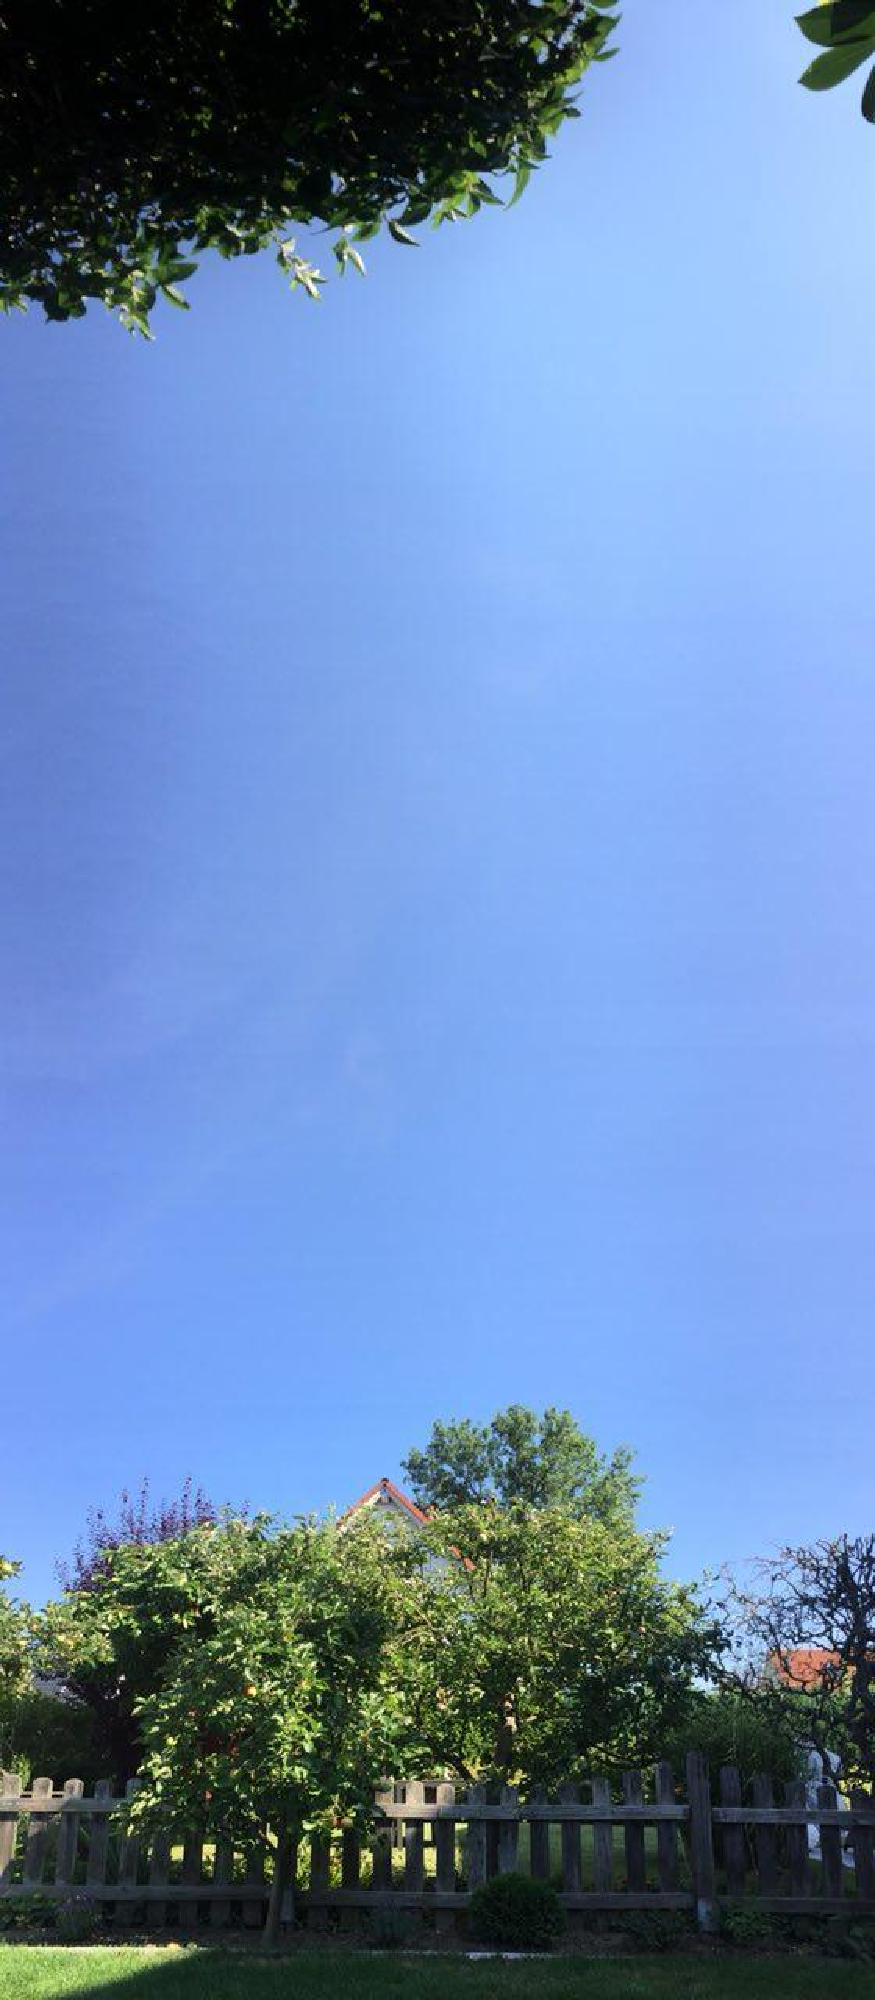
\includegraphics[width=4cm]{./pictures/station_winkel/station_winkel.pdf}
		};
	   \draw[red, line width=0.1cm, rounded corners] (0,2.5cm) rectangle
			   (4cm, 5cm) node[below left, black]{$\Omega_1$};
 	   \draw[red, line width=0.1cm, rounded corners] (0,5.2cm) rectangle
			   (4cm, 7.7cm) node[below left, black]{$\Omega_2$};
 	   \draw[|->, thick] (-0.3,0) node[left]{\SI{0}{\degree}} to ++(0, 9.5cm) node[below left]{\SI{180}{\degree}} node[right]{$\omega$};
\end{tikzpicture}
\end{document}

